\documentclass[11pt,a4paper]{article}
\usepackage[utf8]{inputenc}
\usepackage{amsmath,amssymb}
\usepackage{graphicx}
\usepackage{booktabs}
\usepackage{geometry}
\usepackage{float}
\geometry{margin=1in}
\setlength{\emergencystretch}{3em}

\title{\textbf{Kimchi Premium and Triangular Arbitrage Dislocation Dynamics}\\Draft v1.3}
\author{Songgun Lee \\ \textit{Department of Physics, UC Santa Barbara}}
\date{As of April 2026}

\begin{document}
\maketitle
\begin{abstract}
This study evaluates minute-level triangular arbitrage dislocations in KRW-linked crypto routing using a 141,200-row export across ADA, DOGE, ETH, SOL, and XRP. Forward and reverse directions are analyzed separately, then aggregated into both a best-per-minute-per-asset series and a global best-per-minute series. Under the Upbit fee schedule, threshold-clearing opportunities are found to be extremely rare and absent under stricter reserved-order and USDT/BTC-equivalent 3-leg friction assumptions. The evidence supports a high short-horizon market-efficiency interpretation for this execution setting.
\end{abstract}
\tableofcontents
\newpage

\section{Research Question}
The central research question is: \emph{Does external macroeconomic dislocation (kimchi-premium volatility) induce exploitable internal microstructural inefficiency within a fiat-isolated exchange order book?}

\noindent
The empirical test is built around fee-aware tail-event frequency above execution barrier $V_0$, with direction-separated and best-direction aggregation layers designed to avoid overstating exploitable edge.

\section{Executive Summary}
\begin{itemize}
    \item Dataset scale: 141,200 rows, 5 assets, minute buckets over approximately 10 days.
    \item Objective: test whether observed dislocations survive realistic 3-leg fee hurdles.
    \item Main result: profitability tails are thin; positive net-profit minutes are rare even after best-direction selection.
    \item Fee-consistent result: events above the baseline execution barrier $V_0=0.35\%$ are not observed in this sample, and therefore also not observed for stricter barriers.
\end{itemize}

\section{Contributions}
Relative to a typical dashboard-style arbitrage note, this draft contributes:
\begin{enumerate}
    \item A fee-aware execution framing tied directly to the Upbit schedule (KRW general, KRW reserved, USDT/BTC-equivalent 3-leg thresholds).
    \item A hierarchical analysis protocol: direction-separated to best-per-asset-per-minute, then global best-per-minute.
    \item Explicit negative-result reporting: threshold-clearing rarity is quantified, not inferred.
    \item A reproducible paper pipeline (CSV $\rightarrow$ scripts $\rightarrow$ figures/tables $\rightarrow$ LaTeX PDF).
\end{enumerate}

\section{Instrument and Data}
\begin{itemize}
    \item Source file: \texttt{arb\_data\_export.csv}
    \item Time range (UTC): 2026-04-08 10:46:00 to 2026-04-18 07:40:00
    \item Rows: $N = 141{,}200$
    \item Assets: ADA, DOGE, ETH, SOL, XRP
    \item Directions: Forward / Reverse
    \item Core fields: \texttt{avg\_kimchi}, \texttt{max\_profit}, \texttt{min\_profit}, \texttt{tick\_count}
\end{itemize}

\subsection*{Data Engineering Notes}
\begin{itemize}
    \item \texttt{avg\_kimchi}: 1-minute arithmetic mean of percentage divergence between Upbit KRW and Binance USDT mid-prices, adjusted by live KRW/USD FX.
    \item Exchange server timestamps are aligned post-hoc to reduce local hardware/network latency contamination.
    \item XRP row deficit relative to other assets is treated as likely exchange-side websocket rate-limiting / transient packet loss during high-volume intervals.
\end{itemize}

\section{Definitions}
For minute bucket $t$, asset $a$, and direction $d \in \{F,R\}$:
\begin{align}
K_{t,a,d} &= \text{avg kimchi premium (\%)} \\
\Pi_{t,a,d} &= \text{max triangular net profit (\%)}
\end{align}

Best-of-both per-minute per-asset:
\begin{equation}
\Pi^{\star}_{t,a} = \max\left(\Pi_{t,a,F}, \Pi_{t,a,R}\right)
\end{equation}

Global best-of-minute:
\begin{equation}
\Pi^{\star}_{t} = \max_{a,d}\Pi_{t,a,d}
\end{equation}

Forward route:
\begin{equation}
\mathrm{KRW} \rightarrow \mathrm{BTC} \rightarrow \mathrm{ALT} \rightarrow \mathrm{KRW}
\end{equation}
Reverse route:
\begin{equation}
\mathrm{KRW} \rightarrow \mathrm{ALT} \rightarrow \mathrm{BTC} \rightarrow \mathrm{KRW}
\end{equation}

Forward profit mapping used in the edge-node implementation:
\begin{equation}
M = \left(\frac{1}{P^{ask}_{BTC/KRW}}\right)\left(\frac{1}{P^{ask}_{ALT/BTC}}\right)P^{bid}_{ALT/KRW} - 1
\end{equation}
Execution mode is pure taker (immediate spread crossing); queue and slippage are excluded from baseline and treated as additional real-world friction.

\section{Execution Friction Assumption}
Using the Upbit fee guide provided by the author:
\begin{itemize}
    \item KRW market, general order: Maker/Taker = $0.05\%$
    \item KRW market, reserved maker: $0.139\%$
    \item BTC/USDT market, general order: Maker/Taker = $0.25\%$
\end{itemize}

For a 3-leg triangular execution, the route-level fee barriers are:
\begin{equation}
\tau_{\mathrm{KRW-KRW-BTC}} = 0.05\% + 0.25\% + 0.05\% = 0.35\%
\end{equation}
\begin{equation}
\tau_{\mathrm{KRW,reserved,all\;legs}} = 3 \times 0.139\% = 0.417\%
\end{equation}
\begin{equation}
\tau_{\mathrm{USDT/BTC}} = 3 \times 0.25\% = 0.75\%
\end{equation}

Primary tail metric in this draft is event frequency above $V_0=0.35\%$.

\section{Methodology}
The analysis is performed in three layers:
\begin{enumerate}
    \item \textbf{Direction-separated layer}: evaluate $\Pi_{t,a,F}$ and $\Pi_{t,a,R}$ independently to capture directional asymmetry.
    \item \textbf{Asset-level best-direction layer}: compute $\Pi^\star_{t,a}$ to represent best feasible routing direction per minute for each asset.
    \item \textbf{Global best-minute layer}: compute $\Pi^\star_t$ as an optimistic upper envelope across all assets and directions.
\end{enumerate}
This structure intentionally tests both realistic directional execution and an optimistic upper-bound case, reducing the chance of overstating tradable edge.

\section{Hypotheses and Test Outcomes}
We define three empirical hypotheses for this sample window:
\begin{itemize}
    \item \textbf{H1 (Direction asymmetry):} Forward and reverse routes differ materially in realized edge distribution.
    \item \textbf{H2 (Executable-edge rarity):} Even optimistic best-minute aggregation rarely clears realistic fee thresholds.
    \item \textbf{H3 (Kimchi monotonicity):} Higher kimchi-premium regimes do not guarantee higher fee-cleared opportunity rates.
\end{itemize}

\noindent\textbf{Observed outcomes in this sample:}
\begin{itemize}
    \item H1 supported: forward mean exceeds reverse mean (less negative) and has higher positive-event frequency.
    \item H2 strongly supported: zero exceedance at $V_0=0.35\%$, with zero exceedance also observed at $0.417\%$ and $0.75\%$ for global best-minute.
    \item H3 supported: bin-wise results show no robust monotone increase in fee-cleared rates as kimchi premium rises.
\end{itemize}

\section{Summary Statistics}

\subsection{By Asset and Direction}
\begin{table}[H]
\centering
\caption{Direction-separated profitability summary}
\begin{tabular}{l l r r r r r r r}
\toprule
Asset & Dir & $N$ & Mean & Std & Min & Max & $P(\Pi>0)$ & $P(\Pi>V_0)$ \\
\midrule
ADA & F & 14210 & -1.3877 & 0.6441 & -4.0253 & 0.1522 & 0.000633 & 0.000000 \\
ADA & R & 14210 & -1.5917 & 0.7930 & -4.5642 & -0.1922 & 0.000000 & 0.000000 \\
DOGE & F & 14210 & -1.4591 & 0.3912 & -2.7039 & -0.1189 & 0.000000 & 0.000000 \\
DOGE & R & 14210 & -1.6219 & 0.3200 & -2.3922 & -0.3843 & 0.000000 & 0.000000 \\
ETH & F & 14210 & -0.6900 & 0.1377 & -1.1212 & 0.1256 & 0.000422 & 0.000000 \\
ETH & R & 14210 & -0.7040 & 0.1125 & -0.9426 & 0.1380 & 0.000141 & 0.000000 \\
SOL & F & 14210 & -0.8059 & 0.2668 & -2.0355 & 0.0287 & 0.000211 & 0.000000 \\
SOL & R & 14210 & -0.7247 & 0.1567 & -1.1677 & 0.0207 & 0.000070 & 0.000000 \\
XRP & F & 14210 & -0.4987 & 0.2191 & -1.2628 & 0.0399 & 0.001267 & 0.000000 \\
XRP & R & 13310 & -0.6181 & 0.1873 & -0.9696 & 0.2545 & 0.000075 & 0.000000 \\
\bottomrule
\end{tabular}
\end{table}

\subsection{Best-of-Both Aggregates}
\begin{table}[H]
\centering
\caption{Best-of-both and global-best minute aggregates}
\resizebox{\textwidth}{!}{
\begin{tabular}{l r r r r r r r}
\toprule
Series & $N$ & Mean & Std & Min & Max & $P(\Pi>0)$ & $P(\Pi>V_0)$ \\
\midrule
$\Pi^\star_{t,a}$ (best per-minute per-asset) & 71050 & -0.8122 & 0.4171 & -2.4768 & 0.2545 & 0.000563 & 0.000000 \\
$\Pi^\star_t$ (global best per-minute) & 14210 & -0.3654 & 0.1561 & -0.7986 & 0.2545 & 0.002815 & 0.000000 \\
\bottomrule
\end{tabular}
}
\end{table}

\section{Distributional Properties of Global Best-Minute Profit}
Let $\Pi_t^\star$ denote the global best-per-minute series. Empirical moments for this sample:
\begin{itemize}
    \item Mean: $-0.3654\%$
    \item Standard deviation: $0.1561\%$
    \item Skewness: $-0.2420$
    \item Quantiles: $q_{0.05}=-0.6521\%$, $q_{0.50}=-0.3531\%$, $q_{0.95}=-0.1212\%$
\end{itemize}
All central quantiles remain negative, reinforcing the high-efficiency interpretation under this execution model.

\section{Persistence and Short-Lag Dependence}
The lag-1 autocorrelation of $\Pi_t^\star$ is:
\begin{equation}
\mathrm{ACF}(1) \approx 0.9332
\end{equation}
This indicates strong minute-to-minute persistence in the dislocation state. Given high-frequency overlap and market microstructure continuity, this should be interpreted as state persistence rather than independent repeated arbitrage opportunity.

\section{Direction and Asset-Level Regime Breakdown}
\subsection{Direction-Level}
\begin{table}[H]
\centering
\caption{Forward vs reverse direction statistics}
\begin{tabular}{l r r r}
\toprule
Direction & $N$ & Mean max\_profit (\%) & $P(\Pi>0)$ \\
\midrule
Forward & 71050 & -0.9683 & 0.000507 \\
Reverse & 70150 & -1.0576 & 0.000057 \\
\bottomrule
\end{tabular}
\end{table}

\subsection{Asset-Level}
\begin{table}[H]
\centering
\caption{Asset-level profitability summary}
\begin{tabular}{l r r r}
\toprule
Asset & $N$ & Mean max\_profit (\%) & $P(\Pi>0)$ \\
\midrule
ADA & 28420 & -1.4897 & 0.000317 \\
DOGE & 28420 & -1.5405 & 0.000000 \\
ETH & 28420 & -0.6970 & 0.000281 \\
SOL & 28420 & -0.7653 & 0.000141 \\
XRP & 27520 & -0.5564 & 0.000690 \\
\bottomrule
\end{tabular}
\end{table}

\section{Kimchi Premium Bin Sensitivity}
Using global best-minute observations, kimchi-premium bins are defined and profitability frequencies are computed.
\begin{table}[H]
\centering
\caption{Global best-minute by kimchi-premium regime}
\begin{tabular}{l r r r r}
\toprule
Kimchi bin (\%) & $N$ & Mean (\%) & $P(\Pi>0)$ & $P(\Pi>0.35\%)$ \\
\midrule
$<0$ & 2965 & -0.3873 & 0.007083 & 0.000000 \\
$[0,0.25)$ & 3087 & -0.3666 & 0.001620 & 0.000000 \\
$[0.25,0.5)$ & 4016 & -0.3692 & 0.001743 & 0.000000 \\
$[0.5,0.75)$ & 3147 & -0.3497 & 0.002224 & 0.000000 \\
$\ge 0.75$ & 995 & -0.3305 & 0.000000 & 0.000000 \\
\bottomrule
\end{tabular}
\end{table}
No monotone ``higher-kimchi, higher-executable-edge'' relation appears in this short sample after fee-aware filtering.

\section{Visualization}
\begin{figure}[H]
    \centering
    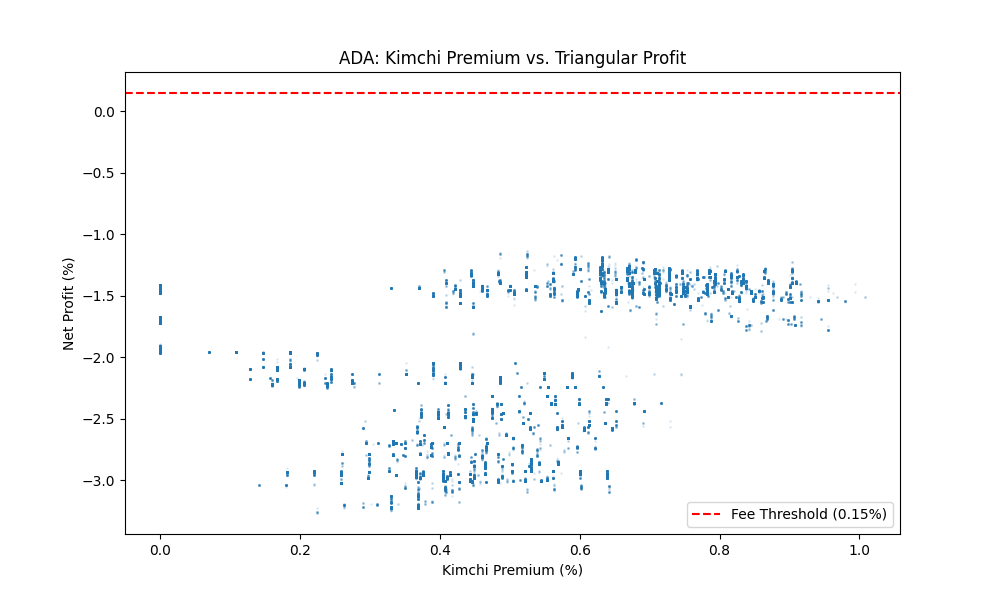
\includegraphics[width=0.95\textwidth]{ada_analysis.png}
    \caption{ADA compressed-history view: Kimchi premium vs. triangular net profit.}
\end{figure}

\begin{figure}[H]
    \centering
    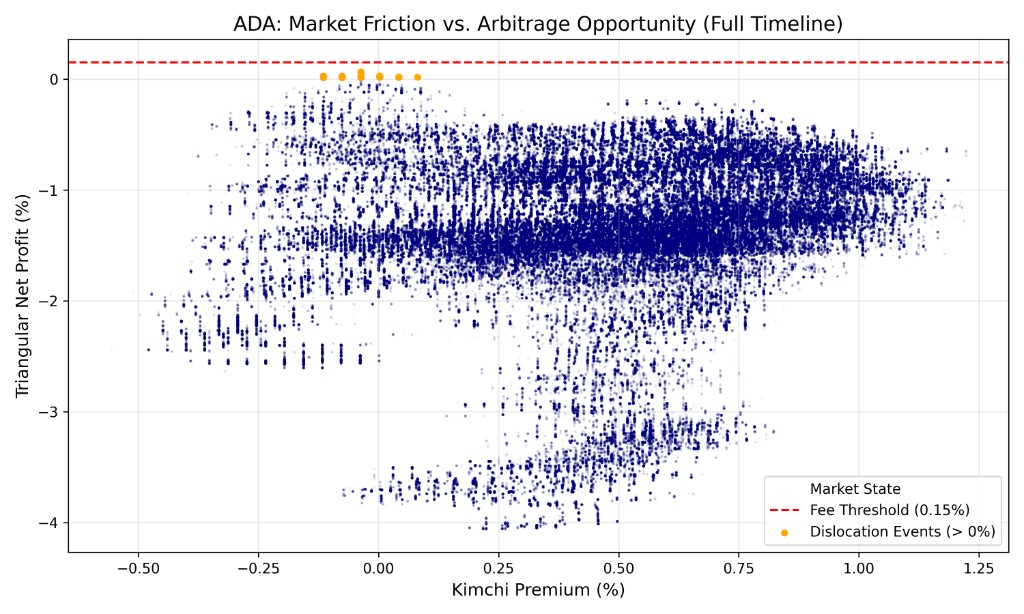
\includegraphics[width=0.95\textwidth]{ada_full_analysis.png}
    \caption{ADA full timeline view with fee threshold and dislocation events.}
\end{figure}

\section{Empirical Finding: High Market Efficiency}
The dominant empirical result is strong execution inefficiency for arbitrage capture (i.e., market \emph{efficiency} against exploitable edge):
\begin{itemize}
    \item Nearly all observations remain below zero net profit after modeled friction.
    \item Even under best-of-both direction selection, positive-minute probability remains very low.
    \item Threshold-clearing events above the baseline barrier $V_0=0.35\%$ are absent in the observed window.
\end{itemize}

For ADA best-of-both minutes, the Kimchi-premium-to-profit linear correlation is:
\begin{equation}
\mathrm{Corr}(K, \Pi^\star) \approx 0.1735
\end{equation}
which indicates only weak monotone linkage in this sample.

\section{Interpretation}
Within this observed period, cross-venue dislocations are mostly absorbed before overcoming execution friction. In practical terms, the market behaves as highly efficient at the minute-level for this strategy specification.

\section{Fee Scenario Sensitivity}
For global best-per-minute profitability $\Pi_t^\star$:
\begin{itemize}
    \item $P(\Pi_t^\star > 0.15\%) = 0.000141$
    \item $P(\Pi_t^\star > 0.35\%) = 0$
    \item $P(\Pi_t^\star > 0.417\%) = 0$
    \item $P(\Pi_t^\star > 0.75\%) = 0$
\end{itemize}
In this sample, opportunities that clear the baseline mixed-leg barrier ($0.35\%$), the KRW reserved-order barrier ($0.417\%$), or the USDT/BTC-equivalent barrier ($0.75\%$) are not observed.

\section{Limitations}
\begin{itemize}
    \item Sample spans roughly 10 days, so regime-level conclusions are preliminary.
    \item Baseline excludes slippage and queue dynamics; practical execution may require $M > 0.40\%$ to survive additional frictions.
    \item Direction-level asymmetries may be influenced by routing constraints not explicitly modeled in this draft.
\end{itemize}

\section{Next Steps}
\begin{enumerate}
    \item Extend to multi-month / multi-regime dataset.
    \item Add exchange-specific fee + slippage decomposition per route (leg-by-leg).
    \item Build conditional models $P(\Pi>\tau \mid K, \text{tick\_count}, a, d)$.
    \item Add event overlays (macro releases, local KRW liquidity shocks).
\end{enumerate}

\appendix
\section{Reproducibility Appendix}
\subsection{File Lineage}
\begin{itemize}
    \item Input data: \texttt{arb\_data\_export.csv}
    \item Plot scripts: \texttt{generate\_plot.py}
    \item Paper generator: \texttt{generate\_paper.py}
    \item White paper source: \texttt{crypto\_kimchi\_draft\_v1.tex}
    \item Output figures: \texttt{ada\_analysis.png}, \texttt{ada\_full\_analysis.png}
    \item Output PDF: \texttt{crypto\_kimchi\_draft\_v1.pdf}
\end{itemize}

\subsection{Suggested Regeneration Workflow}
\begin{verbatim}
# 1) (Optional) regenerate the dynamic paper source from DB export logic
python3 generate_paper.py

# 2) regenerate plots
python3 generate_plot.py

# 3) compile white paper draft (run twice for TOC)
pdflatex -interaction=nonstopmode -halt-on-error crypto_kimchi_draft_v1.tex
pdflatex -interaction=nonstopmode -halt-on-error crypto_kimchi_draft_v1.tex
\end{verbatim}

\subsection{Interpretation Guardrails}
\begin{itemize}
    \item This is a short-window empirical draft, not a full-cycle market invariance claim.
    \item Threshold exceedance depends on route design, queue priority, and unmodeled slippage.
    \item Negative findings remain informative: they constrain where exploitable edge is \emph{not} present.
\end{itemize}

\end{document}

